%% Support sites:
%% http://www.michaelshell.org/tex/ieeetran/
%% http://www.ctan.org/tex-archive/macros/latex/contrib/IEEEtran/
%% and
%% http://www.ieee.org/
%% File list of work: IEEEtran.cls, IEEEtran_HOWTO.pdf, bare_adv.tex,
%%                    bare_conf.tex, bare_jrnl.tex, bare_jrnl_compsoc.tex
% The testflow support page is at:
% http://www.michaelshell.org/tex/testflow/

\documentclass[10pt, conference, compsocconf]{IEEEtran}
% Add the compsocconf option for Computer Society conferences.
%
% If IEEEtran.cls has not been installed into the LaTeX system files,
% manually specify the path to it like:
% \documentclass[conference]{../sty/IEEEtran}
% (max. 10 proceeding pages). 

\usepackage{multirow}
% see http://www.andy-roberts.net/misc/latex/latextutorial4.html

% *** CITATION PACKAGES ***
%
\usepackage{cite}
% cite.sty was written by Donald Arseneau
% V1.6 and later of IEEEtran pre-defines the format of the cite.sty package
% \cite{} output to follow that of IEEE. Loading the cite package will
% result in citation numbers being automatically sorted and properly
% "compressed/ranged". e.g., [1], [9], [2], [7], [5], [6] without using
% cite.sty will become [1], [2], [5]--[7], [9] using cite.sty. cite.sty's
% \cite will automatically add leading space, if needed. Use cite.sty's
% noadjust option (cite.sty V3.8 and later) if you want to turn this off.
% cite.sty is already installed on most LaTeX systems. Be sure and use
% version 4.0 (2003-05-27) and later if using hyperref.sty. cite.sty does
% not currently provide for hyperlinked citations.
% The latest version can be obtained at:
% http://www.ctan.org/tex-archive/macros/latex/contrib/cite/
% The documentation is contained in the cite.sty file itself.

% *** GRAPHICS RELATED PACKAGES ***
%
%\ifCLASSINFOpdf
   \usepackage[pdftex]{graphicx}
  % declare the path(s) where your graphic files are
  % \graphicspath{{../pdf/}{../jpeg/}}
  % and their extensions so you won't have to specify these with
  % every instance of \includegraphics
  % \DeclareGraphicsExtensions{.pdf,.jpeg,.png}
%\else
  % or other class option (dvipsone, dvipdf, if not using dvips). graphicx
  % will default to the driver specified in the system graphics.cfg if no
  % driver is specified.
  % \usepackage[dvips]{graphicx}
  % declare the path(s) where your graphic files are
  % \graphicspath{{../eps/}}
  % and their extensions so you won't have to specify these with
  % every instance of \includegraphics
  % \DeclareGraphicsExtensions{.eps}
%\fi
% graphicx was written by David Carlisle and Sebastian Rahtz. It is
% required if you want graphics, photos, etc. graphicx.sty is already
% installed on most LaTeX systems. The latest version and documentation can
% be obtained at: 
% http://www.ctan.org/tex-archive/macros/latex/required/graphics/
% Another good source of documentation is "Using Imported Graphics in
% LaTeX2e" by Keith Reckdahl which can be found as epslatex.ps or
% epslatex.pdf at: http://www.ctan.org/tex-archive/info/
%
% latex, and pdflatex in dvi mode, support graphics in encapsulated
% postscript (.eps) format. pdflatex in pdf mode supports graphics
% in .pdf, .jpeg, .png and .mps (metapost) formats. Users should ensure
% that all non-photo figures use a vector format (.eps, .pdf, .mps) and
% not a bitmapped formats (.jpeg, .png). IEEE frowns on bitmapped formats
% which can result in "jaggedy"/blurry rendering of lines and letters as
% well as large increases in file sizes.
%
% You can find documentation about the pdfTeX application at:
% http://www.tug.org/applications/pdftex





% *** MATH PACKAGES ***
%
%\usepackage[cmex10]{amsmath}
% A popular package from the American Mathematical Society that provides
% many useful and powerful commands for dealing with mathematics. If using
% it, be sure to load this package with the cmex10 option to ensure that
% only type 1 fonts will utilized at all point sizes. Without this option,
% it is possible that some math symbols, particularly those within
% footnotes, will be rendered in bitmap form which will result in a
% document that can not be IEEE Xplore compliant!
%
% Also, note that the amsmath package sets \interdisplaylinepenalty to 10000
% thus preventing page breaks from occurring within multiline equations. Use:
%\interdisplaylinepenalty=2500
% after loading amsmath to restore such page breaks as IEEEtran.cls normally
% does. amsmath.sty is already installed on most LaTeX systems. The latest
% version and documentation can be obtained at:
% http://www.ctan.org/tex-archive/macros/latex/required/amslatex/math/





% *** SPECIALIZED LIST PACKAGES ***
%
\usepackage{algorithmic}
% algorithmic.sty was written by Peter Williams and Rogerio Brito.
% This package provides an algorithmic environment fo describing algorithms.
% You can use the algorithmic environment in-text or within a figure
% environment to provide for a floating algorithm. Do NOT use the algorithm
% floating environment provided by algorithm.sty (by the same authors) or
% algorithm2e.sty (by Christophe Fiorio) as IEEE does not use dedicated
% algorithm float types and packages that provide these will not provide
% correct IEEE style captions. The latest version and documentation of
% algorithmic.sty can be obtained at:
% http://www.ctan.org/tex-archive/macros/latex/contrib/algorithms/
% There is also a support site at:
% http://algorithms.berlios.de/index.html
% Also of interest may be the (relatively newer and more customizable)
% algorithmicx.sty package by Szasz Janos:
% http://www.ctan.org/tex-archive/macros/latex/contrib/algorithmicx/




% *** ALIGNMENT PACKAGES ***
%
\usepackage{array}
% Frank Mittelbach's and David Carlisle's array.sty patches and improves
% the standard LaTeX2e array and tabular environments to provide better
% appearance and additional user controls. As the default LaTeX2e table
% generation code is lacking to the point of almost being broken with
% respect to the quality of the end results, all users are strongly
% advised to use an enhanced (at the very least that provided by array.sty)
% set of table tools. array.sty is already installed on most systems. The
% latest version and documentation can be obtained at:
% http://www.ctan.org/tex-archive/macros/latex/required/tools/


%\usepackage{mdwmath}
%\usepackage{mdwtab}
% Also highly recommended is Mark Wooding's extremely powerful MDW tools,
% especially mdwmath.sty and mdwtab.sty which are used to format equations
% and tables, respectively. The MDWtools set is already installed on most
% LaTeX systems. The lastest version and documentation is available at:
% http://www.ctan.org/tex-archive/macros/latex/contrib/mdwtools/


% IEEEtran contains the IEEEeqnarray family of commands that can be used to
% generate multiline equations as well as matrices, tables, etc., of high
% quality.


%\usepackage{eqparbox}
% Also of notable interest is Scott Pakin's eqparbox package for creating
% (automatically sized) equal width boxes - aka "natural width parboxes".
% Available at:
% http://www.ctan.org/tex-archive/macros/latex/contrib/eqparbox/





% *** SUBFIGURE PACKAGES ***
\usepackage[tight,footnotesize]{subfigure}
% subfigure.sty was written by Steven Douglas Cochran. This package makes it
% easy to put subfigures in your figures. e.g., "Figure 1a and 1b". For IEEE
% work, it is a good idea to load it with the tight package option to reduce
% the amount of white space around the subfigures. subfigure.sty is already
% installed on most LaTeX systems. The latest version and documentation can
% be obtained at:
% http://www.ctan.org/tex-archive/obsolete/macros/latex/contrib/subfigure/
% subfigure.sty has been superceeded by subfig.sty.



%\usepackage[caption=false]{caption}
%\usepackage[font=footnotesize]{subfig}
% subfig.sty, also written by Steven Douglas Cochran, is the modern
% replacement for subfigure.sty. However, subfig.sty requires and
% automatically loads Axel Sommerfeldt's caption.sty which will override
% IEEEtran.cls handling of captions and this will result in nonIEEE style
% figure/table captions. To prevent this problem, be sure and preload
% caption.sty with its "caption=false" package option. This is will preserve
% IEEEtran.cls handing of captions. Version 1.3 (2005/06/28) and later 
% (recommended due to many improvements over 1.2) of subfig.sty supports
% the caption=false option directly:
%\usepackage[caption=false,font=footnotesize]{subfig}
%
% The latest version and documentation can be obtained at:
% http://www.ctan.org/tex-archive/macros/latex/contrib/subfig/
% The latest version and documentation of caption.sty can be obtained at:
% http://www.ctan.org/tex-archive/macros/latex/contrib/caption/




% *** FLOAT PACKAGES ***
%
%\usepackage{fixltx2e}
% fixltx2e, the successor to the earlier fix2col.sty, was written by
% Frank Mittelbach and David Carlisle. This package corrects a few problems
% in the LaTeX2e kernel, the most notable of which is that in current
% LaTeX2e releases, the ordering of single and double column floats is not
% guaranteed to be preserved. Thus, an unpatched LaTeX2e can allow a
% single column figure to be placed prior to an earlier double column
% figure. The latest version and documentation can be found at:
% http://www.ctan.org/tex-archive/macros/latex/base/



%\usepackage{stfloats}
% stfloats.sty was written by Sigitas Tolusis. This package gives LaTeX2e
% the ability to do double column floats at the bottom of the page as well
% as the top. (e.g., "\begin{figure*}[!b]" is not normally possible in
% LaTeX2e). It also provides a command:
%\fnbelowfloat
% to enable the placement of footnotes below bottom floats (the standard
% LaTeX2e kernel puts them above bottom floats). This is an invasive package
% which rewrites many portions of the LaTeX2e float routines. It may not work
% with other packages that modify the LaTeX2e float routines. The latest
% version and documentation can be obtained at:
% http://www.ctan.org/tex-archive/macros/latex/contrib/sttools/
% Documentation is contained in the stfloats.sty comments as well as in the
% presfull.pdf file. Do not use the stfloats baselinefloat ability as IEEE
% does not allow \baselineskip to stretch. Authors submitting work to the
% IEEE should note that IEEE rarely uses double column equations and
% that authors should try to avoid such use. Do not be tempted to use the
% cuted.sty or midfloat.sty packages (also by Sigitas Tolusis) as IEEE does
% not format its papers in such ways.





% *** PDF, URL AND HYPERLINK PACKAGES ***
%
\usepackage{url}
% url.sty was written by Donald Arseneau. It provides better support for
% handling and breaking URLs. url.sty is already installed on most LaTeX
% systems. The latest version can be obtained at:
% http://www.ctan.org/tex-archive/macros/latex/contrib/misc/
% Read the url.sty source comments for usage information. Basically,
% \url{my_url_here}.





% *** Do not adjust lengths that control margins, column widths, etc. ***
% *** Do not use packages that alter fonts (such as pslatex).         ***
% There should be no need to do such things with IEEEtran.cls V1.6 and later.
% (Unless specifically asked to do so by the journal or conference you plan
% to submit to, of course. )


% correct bad hyphenation here
\hyphenation{op-tical net-works semi-conduc-tor}


\begin{document}
%
% paper title can use linebreaks \\ within to get better formatting as desired
\title{Network Models in the Evaluation of \\ Software Clustering Algorithms}


% author names and affiliations
% use a multiple column layout for up to two different
% affiliations

\author{\IEEEauthorblockN{Rodrigo Souza}
\IEEEauthorblockA{Departamento de Sistemas e Computa\c{c}\~ao \\%line 1 (of Affiliation): dept. name of organization\\
Universidade Federal de Campina Grande \\%line 2: name of organization, acronyms acceptable\\
Campina Grande, Brazil \\%line 3: City, Country\\
rodrigorgs@gmail.com%line 4: Email: name@xyz.com}
%\and
%\IEEEauthorblockN{Authors Name/s per 2nd Affiliation (Author)}
%\IEEEauthorblockA{line 1 (of Affiliation): dept. name of organization\\
%line 2: name of organization, acronyms acceptable\\
%line 3: City, Country\\
%line 4: Email: name@xyz.com}
}
}

% conference papers do not typically use \thanks and this command
% is locked out in conference mode. If really needed, such as for
% the acknowledgment of grants, issue a \IEEEoverridecommandlockouts
% after \documentclass

% for over three affiliations, or if they all won't fit within the width
% of the page, use this alternative format:
% 
%\author{\IEEEauthorblockN{Michael Shell\IEEEauthorrefmark{1},
%Homer Simpson\IEEEauthorrefmark{2},
%James Kirk\IEEEauthorrefmark{3}, 
%Montgomery Scott\IEEEauthorrefmark{3} and
%Eldon Tyrell\IEEEauthorrefmark{4}}
%\IEEEauthorblockA{\IEEEauthorrefmark{1}School of Electrical and Computer Engineering\\
%Georgia Institute of Technology,
%Atlanta, Georgia 30332--0250\\ Email: see http://www.michaelshell.org/contact.html}
%\IEEEauthorblockA{\IEEEauthorrefmark{2}Twentieth Century Fox, Springfield, USA\\
%Email: homer@thesimpsons.com}
%\IEEEauthorblockA{\IEEEauthorrefmark{3}Starfleet Academy, San Francisco, California 96678-2391\\
%Telephone: (800) 555--1212, Fax: (888) 555--1212}
%\IEEEauthorblockA{\IEEEauthorrefmark{4}Tyrell Inc., 123 Replicant Street, Los Angeles, California 90210--4321}}




% use for special paper notices
%\IEEEspecialpapernotice{(Invited Paper)}




% make the title area
\maketitle


\begin{abstract} 

Software modularization recovery algorithms help to understand
how software systems decompose into modules, but they

Software modularization recovery algorithms... bla bla
\end{abstract}

\begin{IEEEkeywords} 
reverse engineering; software modularization; 
empirical evaluation; complex networks;
\end{IEEEkeywords}


% For peer review papers, you can put extra information on the cover
% page as needed:
% \ifCLASSOPTIONpeerreview
% \begin{center} \bfseries EDICS Category: 3-BBND \end{center}
% \fi
%
% For peerreview papers, this IEEEtran command inserts a page break and
% creates the second title. It will be ignored for other modes.
\IEEEpeerreviewmaketitle

\newcommand{\din}[0]{\ensuremath{\delta_{in}}}
\newcommand{\dout}[0]{\ensuremath{\delta_{out}}}

%%%%%%%%%%%%%%%%%%%%%%%%%%%%%%%%%%%%%%%%%%%%%%%%%%%%%%%%%%%%%%%%%%%%%%%%%%%%%%
%%%%%%%%%%%%%%%%%%%%%%%%%%%%%%%%%%%%%%%%%%%%%%%%%%%%%%%%%%%%%%%%%%%%%%%%%%%%%%
%%%%%%%%%%%%%%%%%%%%%%%%%%%%%%%%%%%%%%%%%%%%%%%%%%%%%%%%%%%%%%%%%%%%%%%%%%%%%%

\section{Introduction} \label{sec:introduction}

Large software systems need to be decomposed in modules in order to be
effectively maintained by groups of developers working concurrently. Software
clustering algorithms \cite{Anquetil1999}, also known as architecture recovery
algorithms, find suitable decompositions by analyzing the dependencies between
components in a software system (e.g., classes in object-oriented systems) and
then grouping together highly interdependent components.

Although many software clustering algorithms have been proposed, there is
little empirical evaluation regarding the external quality of the
decompositions they find, i.e., how close the decompositions are from reference
decompositions made by experienced developers \cite{Anquetil1999}. It is
expected that a good algorithm finds decompositions that are similar to
reference decompositions, which can be measured by a similarity metric such as
MoJo or EdgeSim \cite{Mitchell2001}.

Unfortunately, there are few publicly available reference decompositions
\cite{Anquetil1999} and, as a result, there are few studies that compare
software clustering algorithms. Also, because it is costly to obtain reference
decompositions for large systems, most studies test the algorithms with a
couple of small and medium systems \cite{Anquetil1999,Bittencourt2009}.

An alternative approach is to run the algorithms on synthetic, i.e., computer-
generated, component dependency networks with built-in reference
decompositions. This approach enables one to test algorithms with arbitrarily
large samples in a controlled manner. Nevertheless, this approach is often
overlooked, mainly because networks synthesized by naive random network models
are very dissimilar from real component dependency networks.

In this paper, we show that three recently proposed network models are capable
of synthesizing networks that resemble software component dependency networks.
For the sake of simplicity, we limit our analysis to networks of static
dependencies between classes in object-oriented systems written in Java.

The paper is organized as follows: Section \ref{sec:models} summarizes main
characteristics of the three network models.
%
Section \ref{sec:characterization} demonstrates a method to tell if a network
resembles a software component dependency network.
%
Section \ref{sec:evaluation} shows empirically that the three models synthesize
networks that resemble software component dependency networks.
%
Section \ref{sec:conclusion} discusses the impact of this research and future
work.

%%%%%%%%%%%%%%%%%%%%%%%%%%%%%%%%%%%%%%%%%%%%%%%%%%%%%%%%%%%%%%%%%%%%%%%%%%%%%%
%%%%%%%%%%%%%%%%%%%%%%%%%%%%%%%%%%%%%%%%%%%%%%%%%%%%%%%%%%%%%%%%%%%%%%%%%%%%%%
%%%%%%%%%%%%%%%%%%%%%%%%%%%%%%%%%%%%%%%%%%%%%%%%%%%%%%%%%%%%%%%%%%%%%%%%%%%%%%

\section{Network Models} \label{sec:models} 

Network theory studies general properties of many types of networks by using
statistical analysis. Of special interest are the so called scale-free
networks, i.e., networks with a highly heterogeneous distribution of the number
of edges per vertex. Scale-free networks have been found in many domains,
including sociology, biology, technology, linguistics, and software. It has
been found that class dependency networks, represented as directed unweighted
graphs, are scale-free \cite{Myers2003}. Thus, the study of the structure of
object-oriented software systems can benefit from the vast literature available
about scale-free networks.

Scale-free network models are algorithms that can be proven, either formally or
empirically, to synthesize networks that are scale-free. Although many
scale-free network models have been proposed, we were able to find in the
literature only two models that generate networks with built-in modules: CGW
\cite{Chen2008} and LFR \cite{Lancichinetti2009}. Also, we adapted a simple and
flexible model, BCR \cite{Bollobas2003}, to produce modules. We called the new
model BCR+.

The networks generated by the three models are represented as directed
unweighted graphs with modules, which makes them suitable for testing software
clustering algorithms. All models are controllable by a set of parameters,
including number of vertices and number of modules. Parameters specific to each
model influence network characteristics such as number of edges and proportion
of external edges (edges connecting vertices from distinct modules).

%%%%%%%%%%%%%%%%%%%%%%%%%%%%%%%%%%%%%%%%%%%%%%%%%%%%%%%%%%%%%%%%%%%%%%%%%%%%%%
%%%%%%%%%%%%%%%%%%%%%%%%%%%%%%%%%%%%%%%%%%%%%%%%%%%%%%%%%%%%%%%%%%%%%%%%%%%%%%
%%%%%%%%%%%%%%%%%%%%%%%%%%%%%%%%%%%%%%%%%%%%%%%%%%%%%%%%%%%%%%%%%%%%%%%%%%%%%%

\section{Characterization of Software Networks} \label{sec:characterization}

In the remaining of this paper, we will use the expression ``software network''
to refer to a network of static dependencies between classes of a software
system, in contrast to networks studied in other domains.

Our research hypothesis is that at least one of the presented models can
synthesize networks that are similar to software networks. A central issue,
thus, is how to measure similarity between networks.

We already know that the models synthesize networks that, just like software
networks, are scale-free. This single property, though, is insufficient to
prove the hypothesis, since many known scale-free networks are not software
networks (e.g., biologic networks). Therefore, the similarity metric should be
able to distinguish between software and non-software networks.

In this section we present a similarity metric and validate it by applying it
to a data set containing both software and non-software networks. 

%%%%%%%%%%%%%%%%%%%%%%%%%%%%%%%%%%%%%%%%%%%%%%%%%%%%%%%%%%%%%%%%%%%%%%
\subsection{Similarity Between Networks}

In a recent work, Milo et al. \cite{Milo2004} characterized networks by
analyzing their triad concentration. A triad is a network with three vertices
in which all vertices are connected. There are only 13 distinct triads, one for
each possible configuration of directed edges, as shown in Figure
\ref{fig:triads}.

\begin{figure}[t]
\centering
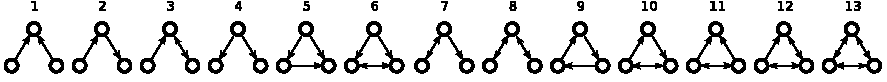
\includegraphics{triads}
%[width=1.0\textwidth]{triads}
\caption{The 13 network triads.}
\label{fig:triads}
\end{figure}

By counting how many times each triad appears in a network, one can build a
triad concentration profile (TCP), which is a vector with 13 numbers that
summarize the local structure of the network. Figure \ref{fig:profiles} shows
the TCP for networks from two distinct domains.

% Word adjacency network: word Y follows word X => X->Y
\begin{figure}[t]
\center
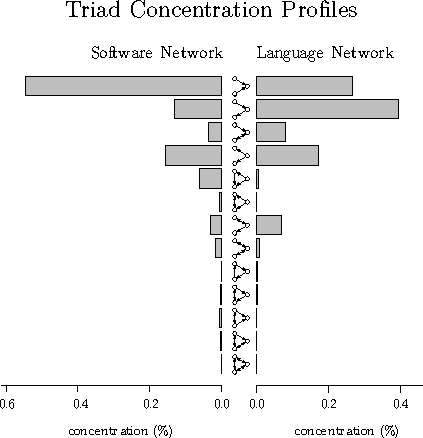
\includegraphics{tcp}
\caption{Triad concentration profiles (TCP) for two networks. On the left,
network extracted from the software system JabRef, version 2.5b2. On the
right, word adjacency network for the Japanese language \cite{Milo2004}.}
\label{fig:profiles}
\end{figure}

Following the work by Milo et al. \cite{Milo2004}, similarity between two
networks is measured by computing Pearson's correlation coefficient between the
corresponding TCPs, which yields a value between -1 (most dissimilar) and 1
(most similar):

$$
\mathrm{similarity}(a, b) ~=~ 
  \mathrm{cor}(\mathrm{TCP}(a), \mathrm{TCP}(b))\mathrm{,}
$$

where $a$ and $b$ are networks, TCP($x$) is the triad concentration profile for
network $x$, and cor($x$, $y$) is Pearson's correlation coefficient.

%%%%%%%%%%%%%%%%%%%%%%%%%%%%%%%%%%%%%%%%%%%%%%%%%%%%%%%%%%%%%%%%%%%%%%
\subsection{Data Set}

To support the evaluation of the metric, we have collected 131 networks from
many different domains. The networks are described in detail at
\url{http://bit.ly/7DPW5X}.

\subsubsection{Software networks} We have collected 65 software systems written
in Java, with size ranging from 111 to 35,363 classes. Java was chosen for
being a popular programming language in which many open source systems have
been written. The software networks, representing static dependencies between
classes, were extracted with the tool Dependency Finder
(\url{http://depfind.sf.net}).

\subsubsection{Non-software networks} We have collected 66 networks from
distinct domains, such as biology, sociology, technology, and linguistics, with
size ranging from 32 to 18,163 vertices. These networks are freely available on
the Internet and have been previously studied in the literature.
% S-score

%%%%%%%%%%%%%%%%%%%%%%%%%%%%%%%%%%%%%%%%%%%%%%%%%%%%%%%%%%%%%%%%%%%%%%
\subsection{Evaluation of the Similarity Metric}

%In order to evaluate the similarity metric, we measured the similarity between
%the networks in the data set. 

For the purposes of this research, a similarity metric must fulfill two
conditions: (i) it must yield high similarity between software networks, and
(ii) it must yield lower similarity between software networks and networks from
other domains.

Using the data set we can define S-score, a metric that represents how much a
particular network resembles software networks. It is defined as the average
similarity between the network and a sample of software networks:

$$
\mathrm{S\mbox{-}score}(a) ~=~ \frac{
\displaystyle\sum_{s \in S} \mathrm{similarity}(a, s)
}{|S|} \mathrm{,}
$$

where $S$ is the set of sample software networks, and $|S|$ is the number of
networks in $S$. In this work we use the full software data set consisting of
65 software networks as our sample.

We used the tool igraph (\url{http://igraph.sf.net/}) to extract the TCP for
each network in the data set. Then, we measured the S-score for each software
network, which ranged from 0.83 to 0.98, with average 0.97 and standard
deviation 0.03. The high average S-score and the low standard deviation show
that the metric successfully characterizes software networks by capturing their
common structural patterns.

Then we measured the S-score for each non-software network. The majority of the
networks (97.0\%) had a S-score lower than 0.83, which is the lowest S-score
for software networks in the sample. Some networks, e.g., the friendship
networks between students, showed negative S-score, meaning that they are very
different from software networks.

Two networks, though, showed high S-score: the network of links between blogs
on politics, with S-score 0.97, and the neural network of the worm C. Elegans,
with S-score 0.88. Further investigation is needed in order to discover the
reasons behind the high values and whether auxiliary metrics can differentiate
these networks from software networks.

\subsection{A Network Classification Model} \label{sec:classmodel} % TODO:
Although the S-score of a network tells how close it is from software networks,
it does not tell whether a network is close enough that it can be considered
software-like. What is needed is a binary classification model that
distinguishes software-like networks from the other networks. The distinction
can be made by choosing a suitable S-score threshold. If a network has a S-score
below the threshold, it is considered dissimilar from software networks;
otherwise, it is considered software-like.

As we have shown on the previous section, there are non-software networks with
high S-scores, hence it is impossible to build a perfect classification model,
regardless of the threshold. Nonetheless, a classification model can be
evaluated by its precision and recall. Consider our data set with both software
and non-software networks. Let $S$ be the set of all software networks, and $L$
the set of all networks that were classified by the model as software-like. The
precision of the model is

$$
\mathrm{precision}: ~\frac{S \cap L}{L},
$$

and the recall is

$$
\mathrm{recall}: ~\frac{S \cap L}{S}.
$$

Increasing the threshold has the effect of reducing the recall, because fewer
software networks are classified as software-like. Decreasing the threshold has
the effect of reducing the precision, because more non-software networks are
classified as software-like. 

The choice of a proper threshold, thus, depends on whether it is more important
to have high precision or high recall. Because our research hypothesis is that
networks synthesized by the presented models are software-like, higher
precision means a stronger test, as fewer networks are classified as
software-like.

To get 100\% precision, the threshold needs to be 0.98, so the non-software
network with highest S-score is below the threshold. But the recall in this
case would be low, because most software networks would be misclassified, so we
chose the value 0.88, that is immediately above the second greater S-score for
a non-software network. With this value, we have both high recall (95.4\%) and
high precision (96.9\%).

%%%%%%%%%%%%%%%%%%%%%%%%%%%%%%%%%%%%%%%%%%%%%%%%%%%%%%%%%%%%%%%%%%%%%%%%%%%%%%
%%%%%%%%%%%%%%%%%%%%%%%%%%%%%%%%%%%%%%%%%%%%%%%%%%%%%%%%%%%%%%%%%%%%%%%%%%%%%%
%%%%%%%%%%%%%%%%%%%%%%%%%%%%%%%%%%%%%%%%%%%%%%%%%%%%%%%%%%%%%%%%%%%%%%%%%%%%%%

\section{Evaluation of Network Models} \label{sec:evaluation}

In the previous section it was shown that many networks, although scale-free,
can be distinguished from software networks by a simple classification model
based on triad concentration profiles. In this section we show empirically that
the three network models previously presented can synthesize networks that are
indistinguishable from software networks. The experiment consists of
synthesizing networks using many combinations of parameters from the three
models, and then classifying each network as software-like or non
software-like. 

Because the possible combinations of parameter values are infinite, we have set
the number of vertices to 1000 and then varied the remaining parameters in
discrete steps. The number of modules varied between 2, 4, 8, 16, and 32. For
each of the remaining model-specific parameters, at least 3 values were chosen.
When possible, the values were chosen to cover the entire parameter domain. In
the case of unbound parameters, the values were chosen to approximate
characteristics of the networks in the software network data set. In total,
9,500 networks were generated with the BCR+ model, 38,790 with the CGW model,
and 1,296 with the LFR model.

\subsection{Results}

Each synthesized network was classified as software-like or non software-like,
using the classification model presented in Section \ref{sec:classmodel}. The
results are summarized in Table \ref{tab:results}. 

\begin{table}
\caption{Results for the classification of synthetic networks}
\centering
\begin{tabular}{|l|l|}
\hline
Model & Networks classified as software-like \\
\hline 
\hline
BCR+ & 21.18\% \\ % 2012 / 9500
\hline
CGW  & 19.40\% \\  % 7524 / 38790
\hline
LFR  & 31.25\% \\ %  405 / 1296
\hline
\end{tabular}
\label{tab:results}
\end{table}

All models synthesized both software-like and non software-like networks. The
proportion of software-like networks was greater than 19\% for all models,
discarding the possibility that this result was obtained by pure chance. (The
specific proportion of software-like networks for each network should not be
interpreted as a measure of quality: with these results we cannot tell whether
one model is better than the others.)

Of course, this result is of little practical value unless there is a
relationship between parameter values and S-score. For the purpose of this
research, it is important to know which values are more likely to lead to
software-like networks.

The algorithm 1R \cite{OneR} from machine learning was used to help discover
such relationship. It analyzes the parameters and the classification of each
network and finds a rule that relates the value of a single parameter with the
classification (software/non-software). Such rules can be evaluated according
to their accuracy, i.e., the proportion of networks that are correctly
classified. The rules found by 1R are shown in Table \ref{tab:rules}.

\begin{table}
\caption{Rules for predicting the classification of a synthetic network. S
stands for software-like and N stands for non software like; $\alpha$, $p_1$, and $\gamma$ are parameters.}
\centering
\begin{tabular}{|l|l|l|}
\hline
Model & Rule & Accuracy \\
\hline 
\hline
\multirow{2}{*}{BCR+}
     & $\alpha \ge 0.7 \Rightarrow S$ & \multirow{2}{*}{82.4\%}  \\ 
     & $\alpha < 0.7 \Rightarrow N$ & \\ 
\hline
\multirow{2}{*}{CGW}
     & $p_1 \ge 0.5 \Rightarrow S$ & \multirow{2}{*}{82.3\%} \\  
     & $p_1 < 0.5 \Rightarrow N$ & \\  
\hline
\multirow{2}{*}{LFR}   
     & $\gamma < 2.44 \Rightarrow S$ & \multirow{2}{*}{78.9\%} \\ 
     & $\gamma \ge 2.44 \Rightarrow N$ & \\ 
\hline
\end{tabular}
\label{tab:rules}
\end{table}

The rules are very simple and, thus, easy to follow. Despite their simplicity,
they have high accuracy, approximately 80\% for all models.  

%%%%%%%%%%%%%%%%%%%%%%%%%%%%%%%%%%%%%%%%%%%%%%%%%%%%%%%%%%%%%%%%%%%%%%%%%%%%%%
%%%%%%%%%%%%%%%%%%%%%%%%%%%%%%%%%%%%%%%%%%%%%%%%%%%%%%%%%%%%%%%%%%%%%%%%%%%%%%
%%%%%%%%%%%%%%%%%%%%%%%%%%%%%%%%%%%%%%%%%%%%%%%%%%%%%%%%%%%%%%%%%%%%%%%%%%%%%%

\section{Conclusion and Future Work} \label{sec:conclusion}
% revised 2009-09-03

We have shown empirically that network models found in the literature can
synthesize networks that resemble the network of static dependencies between
classes in object-oriented systems. This result supports the use of synthetic
networks in the evaluation of software clustering algorithms.
%that operate on class dependency networks. 

The use of synthetic data is common in distributed computing research, but
still underexplored in software engineering research. Because many reverse
engineering tasks rely on dependency data, we expect this
work to have impact beyond the software clustering community.

We accept that it is important to evaluate the algorithms with real software
networks, but we argue that the use of synthetic networks in a complementary
manner can give researchers new insights about the algorithms. First, the use
of models allows the creation of large test sets, thus diminishing the small
sample effects. Moreover, the networks are created in a controlled way,
according to model parameters, so it is possible to study the behavior of the
algorithms with different parameter values.

In a future work, we intend to use synthetic networks in the evaluation of
software clustering algorithms that were previously tested with real networks.
After that we will be able to compare the results obtained by the two
approaches.

% Also, it is worth investigating models that account for more than one type
% of dependency.




% An example of a floating figure using the graphicx package.
% Note that \label must occur AFTER (or within) \caption.
% For figures, \caption should occur after the \includegraphics.
% Note that IEEEtran v1.7 and later has special internal code that
% is designed to preserve the operation of \label within \caption
% even when the captionsoff option is in effect. However, because
% of issues like this, it may be the safest practice to put all your
% \label just after \caption rather than within \caption{}.
%
% Reminder: the "draftcls" or "draftclsnofoot", not "draft", class
% option should be used if it is desired that the figures are to be
% displayed while in draft mode.
%
%\begin{figure}[!t]
%\centering
%\includegraphics[width=2.5in]{myfigure}
% where an .eps filename suffix will be assumed under latex, 
% and a .pdf suffix will be assumed for pdflatex; or what has been declared
% via \DeclareGraphicsExtensions.
%\caption{Simulation Results}
%\label{fig_sim}
%\end{figure}

% Note that IEEE typically puts floats only at the top, even when this
% results in a large percentage of a column being occupied by floats.


% An example of a double column floating figure using two subfigures.
% (The subfig.sty package must be loaded for this to work.)
% The subfigure \label commands are set within each subfloat command, the
% \label for the overall figure must come after \caption.
% \hfil must be used as a separator to get equal spacing.
% The subfigure.sty package works much the same way, except \subfigure is
% used instead of \subfloat.
%
%\begin{figure*}[!t]
%\centerline{\subfloat[Case I]\includegraphics[width=2.5in]{subfigcase1}%
%\label{fig_first_case}}
%\hfil
%\subfloat[Case II]{\includegraphics[width=2.5in]{subfigcase2}%
%\label{fig_second_case}}}
%\caption{Simulation results}
%\label{fig_sim}
%\end{figure*}
%
% Note that often IEEE papers with subfigures do not employ subfigure
% captions (using the optional argument to \subfloat), but instead will
% reference/describe all of them (a), (b), etc., within the main caption.


% An example of a floating table. Note that, for IEEE style tables, the 
% \caption command should come BEFORE the table. Table text will default to
% \footnotesize as IEEE normally uses this smaller font for tables.
% The \label must come after \caption as always.
%
%\begin{table}[!t]
%% increase table row spacing, adjust to taste
%\renewcommand{\arraystretch}{1.3}
% if using array.sty, it might be a good idea to tweak the value of
% \extrarowheight as needed to properly center the text within the cells
%\caption{An Example of a Table}
%\label{table_example}
%\centering
%% Some packages, such as MDW tools, offer better commands for making tables
%% than the plain LaTeX2e tabular which is used here.
%\begin{tabular}{|c||c|}
%\hline
%One & Two\\
%\hline
%Three & Four\\
%\hline
%\end{tabular}
%\end{table}


% Note that IEEE does not put floats in the very first column - or typically
% anywhere on the first page for that matter. Also, in-text middle ("here")
% positioning is not used. Most IEEE journals/conferences use top floats
% exclusively. Note that, LaTeX2e, unlike IEEE journals/conferences, places
% footnotes above bottom floats. This can be corrected via the \fnbelowfloat
% command of the stfloats package.

% conference papers do not normally have an appendix


% use section* for acknowledgement
\section*{Acknowledgment}

Dalton, Jorge, Christina, Garcia, Charles, Fabiola, Italo, Roberto, Jemerson,
Sandra, and Lancichinetti.

% trigger a \newpage just before the given reference
% number - used to balance the columns on the last page
% adjust value as needed - may need to be readjusted if
% the document is modified later
%\IEEEtriggeratref{8}
% The "triggered" command can be changed if desired:
%\IEEEtriggercmd{\enlargethispage{-5in}}

% references section

% can use a bibliography generated by BibTeX as a .bbl file
% BibTeX documentation can be easily obtained at:
% http://www.ctan.org/tex-archive/biblio/bibtex/contrib/doc/
% The IEEEtran BibTeX style support page is at:
% http://www.michaelshell.org/tex/ieeetran/bibtex/
\bibliographystyle{IEEEtran}
% argument is your BibTeX string definitions and bibliography database(s)
%\bibliography{IEEEabrv,../bib/paper}
\bibliography{paper1}
%
% <OR> manually copy in the resultant .bbl file
% set second argument of \begin to the number of references
% (used to reserve space for the reference number labels box)
%\begin{thebibliography}{1}
%
%\bibitem{IEEEhowto:kopka}
%H.~Kopka and P.~W. Daly, \emph{A Guide to \LaTeX}, 3rd~ed.\hskip 1em plus
%  0.5em minus 0.4em\relax Harlow, England: Addison-Wesley, 1999.
%
%\end{thebibliography}

% that's all folks
\end{document}


